\section{Ziel}
In deisem Experiment soll der Faraday Effekt in GaAs gemessen werden.
\section{Theorie}
\label{sec:Theorie}
\subsection{Bandstruktur und effektive Masse}
Die Verteilung von Elektronen in Festkörpern wird üblicherweise durch die sogenannte Bandstruktur dargestellt und soll hier noch einmal kurz wiederholt werden.
Grundsätzlich unterscheidet man bei Festkörpern zwischen Metallen, Halbleitern und Isolatoren.
Jede Art von Festkörper besitzt ein Leitungsband in dem sich die Leitungselektronen befinden und Valenzbänder für die Valenzelektronen.
Die verschiedenen Festkörper unterscheiden sich in der Bandstruktur durch die verschieden großen Abstände zwischen Leitungs und Valenzbändern, siehe Abbildung \ref{fig:bandstruk}.
Bei metallen liegt die Fermi Energie in dem Leitungsband und die Bandlücke zwischen Leitungs- und Valenzband ist relativ klein, daher sind Metalle gute elektrische Leiter.
Bei Halbleitern und bei Isolatoren liegt die Fermienergie in der Bandlücke zwischen Leitungs und Valenzband. 
Isolatoren haben die größte Bandlücke und sind damit auch die schlechtesten elektrischen Leiter. 
Bei Halbleitern ist die Bandlücke relativ klein und für die Elektronen gut überwindbar.
\begin{figure}[ht]
    \centering
    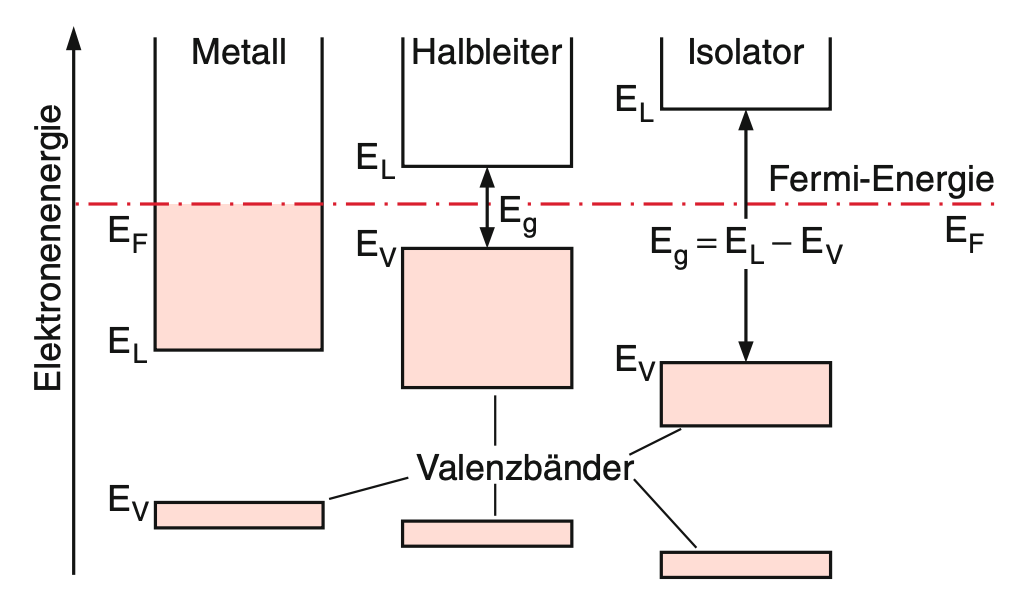
\includegraphics[scale = 0.5]{./bilder/Bandstruktur_demtroeder.png}
    \caption{Chematische Darstellung der Bandstruktur von Isolatoren und Leitern \cite{demtröder}}
    \label{fig:bandstruk}
\end{figure}

Um Elektronen im Festkörper zu beschreiben ist zu beachten, dass das Elektron nicht nur ein elektrisches Potential erfährt sondern zusätzlich noch von einem ortsabhängigem Potential beeinflusst wird.
Damit die Elektronen weiterhin als freie Elektronen beschrieben werden können modifiziert man ihre Masse zu einer effektiven Masse $m^{\*}$ die das Kristallpotential mit beachtet.

Die beschleunigung eines Elektrons in einem Festkörper lässt sich als Ableitung der Gruppengeschwindigkeit definieren:
\begin{equation}
    \vec{a} = \frac{\text{d}v_g}{\text{d}t} = \frac{1}{\hbar} \left( \frac{\text{d}^2 E}{\text{d}k^2}\right) \cdot \frac{\text{d}\vec{k}}{\text{d}t}
    \label{eqn:bewegungsgl}
\end{equation}
Wobei in Gleichung \ref{eqn:bewegungsgl} die Ableitung des Impulses nach der Zeit als Kraft geteilt durch das Plancksche Wirkungsquantum ausgedrückt werden kann.
\begin{equation}
    \vec{a} = \frac{1}{\hbar^2} \left( \frac{\text{d}^2 E}{\text{d}k^2}\right) \cdot \vec{F}
\end{equation}

Diese Formel ist kann nun als Bewegungsgleichung für die freien Elektronen betrachtet werden:
\begin{align}
    \vec{a} &= \frac{1}{m^{*}} \vec{F}\\
    m^{*} &= \hbar^2 \left( \frac{\text{d}^2 E}{\text{d}k^2}\right)^{-1}
\end{align}

\subsection{Dotierung von Halbleitern}
Die Dotierung von Halbleitern meint das Einfügen von Fremdatomen in das bestehende Kristallgitter um die Bandstruktur und damit auch die Leitfähigkeit des Kristalls zu verändern.
Es wird bei der Dotierung zwischen Donatoren und Akzeptoren unterschieden.
Wir betrachten hier beispielsweise einen Halbleiter mit 4-wertigen Atomen.

\subsubsection{n-Dotierung}
Als n-Dotierung bezeichnet man nun das hinzufügen von 5-wertigen Atomen in den Halbleiter.
Durch die 5-wertigkeit der neuen Atome ist jeweils eines ihrer Leitungsatome nur sehr schwach gebunden und kann als weiteres Leitungselektron fungieren.
Dieser neue Zustand für die Elektronen wird Donatorzustand genannt und befindet sich knapp unter der Fermi Energie.
Durch die nähe des Zustands zum Leitungsband, können schon kleine Energien das Elektron in das Leitungsband befördern.
\begin{figure}[ht]
    \centering
    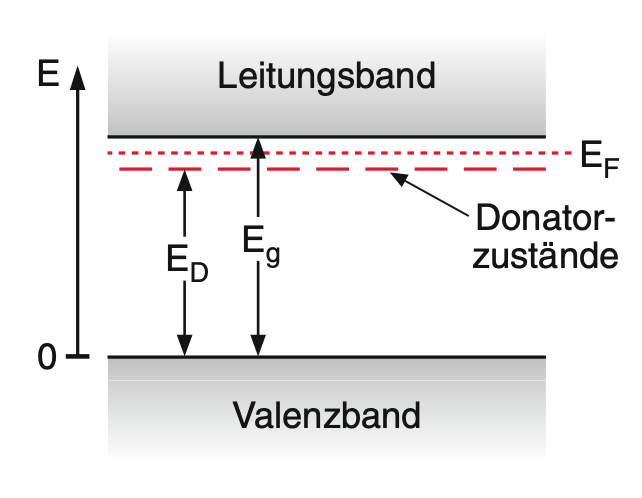
\includegraphics[scale = 0.5]{./bilder/n_Donatorschema_demtroeder.png}
    \caption{Der Donatorzustand in einem n-dotierten Halbleiter \cite{demtröder}.}
    \label{fig:n_donator}
\end{figure}

\subsubsection{p-Donatoren}

Werden dem Halbleiter niedrigwertige, zum Beispiel 3-wertige, Atome hinzugefügt, spricht man von einem p-dotierten Halbleiter. In p-dotierten Halbleitern entsteht auch ein neuer Zustand, der Akzeptorzustand, da die neuen Atome ein Atom zu wenig haben um Bindungen mit den anderen Atomen einzugehen.
Der Akzeptorzustand liegt über dem Valenzband knapp über der Fermi Energie.
Durch die nähe zum Valenzband können Elektronen schon durch geringe Energiemengen über die Fermienergie gehoben werden und sogenannte Löcher im Valenzband hinterlassen.
Die Löcher im Valenzband können als quasi-Ladungsträger die Leitfähigkeit des Halbleiters erhöhen.
\begin{figure}[ht]
    \centering
    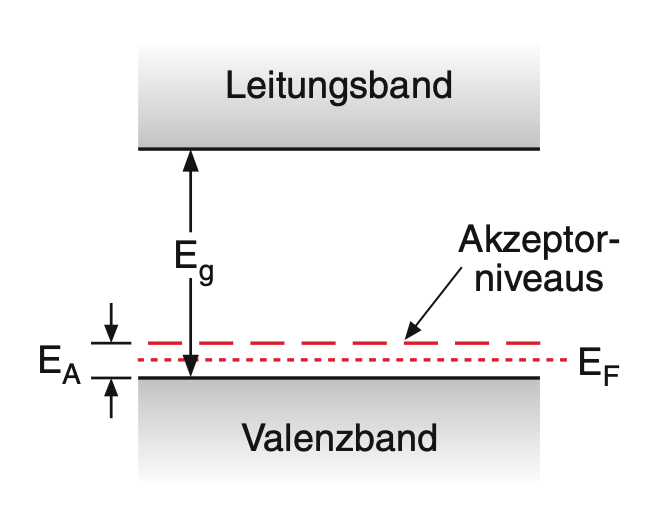
\includegraphics[scale = 0.5]{./bilder/p_Donatorschema_demtroeder.png}
    \caption{Der Akzeptorzustand in einem p-dotierten Halbleiter \cite{demtröder}.}
    \label{fig:p_donator}
\end{figure}

\subsection{Faraday Effekt}
Der Faraday Effekt beschreibt die Rotation der Polarisationsebene eines Lichtstrahls beim Durchlaufen einer !!Probe!! in einem Magnetfeld.

\subsection{Zirkulare Doppelbrechung}
Polarisationsebene eines linear polarisierten Lichtstrahls wird beim durchlaufen eines Kristalls gedreht.
\begin{equation}
    \vec{P} = \epsilon_0 \underline{\underline{\Xi}} \vec{E}
\end{equation}

\begin{equation}
    \underline{\underline{\Xi}} = 
    \begin{pmatrix}
        \Xi_{xx} & i \Xi_{xy} & 0\\
        -i \Xi_{xy} & \Xi_{xx} & 0\\
        0 & 0 & \Xi_{zz}\\
    \end{pmatrix}
\end{equation}

\begin{equation}
    \nabla \times \left( \nabla \times \vec{E} \right) = -\frac{1}{c^2} \left( 1 + \underline{\underline{\Xi}} \right) \cdot \frac{\partial^2 \vec{E}}{\partial t^2}
\end{equation}

\begin{equation}
    \frac{\omega^2}{c^2} \cdot E_z = \frac{\omega^2}{c^2} \Xi_{zz} \cdot E_z
\end{equation}



\subsection{Bestimmung der Effektiven Masse}